{\tabulinesep=1mm
\begin{tabu}{|p{16cm} |}
\hline 
\textbf{The Halting Problem:} Does a given program ever halt when executed 
on a given input? This given input has to be general. \\
\begin{center}
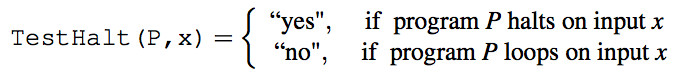
\includegraphics[width=10cm, height=1cm]{intro_testhalt.jpg}
\end{center}

How do we prove that \texttt{TestHalt} does not exist? Let'��s assume that it does, 
and hope we reach a contradiction. \newline
Define another program:
\begin{center}
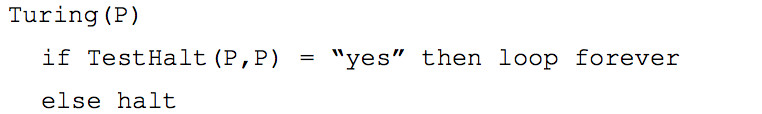
\includegraphics[width=10cm, height=1.5cm]{intro_turing.jpg}
\end{center}
What happens when we call \texttt{Turing(Turing)}?
\begin{description}
\item[Case 1]: It halts.
If \texttt{Turing(Turing)} halts then \texttt{TestHalt(Turing, Turing)} 
must have returned no. But \texttt{TestHalt(Turing Turing)} calls 
\texttt{Turing(Turing)} and calling \texttt{Turing(Turing)} must loop. 
But we assumed that \texttt{Turing(Turing)} halted. Contradiction.
\item[Case 2]: It loops.
This implies that \texttt{TestHalt(Turing, Turing)} returned yes, which by the 
way that \texttt{TestHalt} is defined implies that \texttt{Turing} halted. 
But we assumed  that \texttt{Turing(Turing)} looped. Contradiction.
\end{description}
\\
\hline
\end{tabu}
}

\fbox{\begin{minipage}{16.3cm}
How is this just a reformulation of proof by diagonalization?
\begin{center}
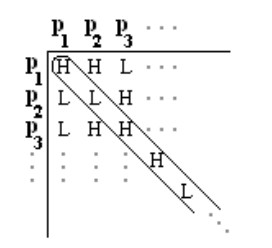
\includegraphics[width=4.5cm, height=4cm]{intro_diagonal.jpg}
\end{center}
List all possible programs as rows and columns. The rows are the programs 
and the columns are the inputs. Turing must be one of the rows, say row $n$. 
If entry $(n, n) $ is $H$ then Turing will loop by definition. If entry 
$(n, n)$ is $L$ then Turing will halt by definition. Therefore Turing 
cannot be on the list of all programs and therefore it does not exist. Therefore the Halting Problem is unsolvable. We can use this to prove 
that other problems are also unsolvable. \newline
Say we are asked if program $M$
is solvable. To prove it is not, we just need to prove the following claim: 
If we can compute program $M$, then we could also compute the halting problem. This would then prove that $M$ can not exist, since the halting problem 
is not computable. This amounts to proof by contradiction.
\end{minipage}}